%
% $Id: report.tex 52 2011-10-03 17:08:43Z justinkamerman $ 
%
% $LastChangedDate: 2011-10-03 14:08:43 -0300 (Mon, 03 Oct 2011) $ 
% 
% $LastChangedBy: justinkamerman $
%

\documentclass[10pt]{article}
\usepackage{graphicx}
\usepackage{algorithm}
\usepackage{algorithmic}
\usepackage{wrapfig}
\usepackage{caption3} % load caption package kernel first
\DeclareCaptionOption{parskip}[]{} % disable "parskip" caption option
\usepackage[font=small,format=plain,labelfont=bf,up,textfont=it,up]{caption}



\title{Document Indexing Using Aho-Corasick State Machines}
\author{Damien DuBois, Justin Kamerman, Ramanpreet Singh}
\date{\today}

\begin{document}
\maketitle

%----------------------------------------
% Abstract
%----------------------------------------
\begin{abstract}
The Aho-Corasick algorithm was originally proposed as a bibliographic
search mechanism, efficient enough to preclude the construction and
maintenance of a search index. As the size of document collections
have grown since the development of the algorithm, document
collections have grown to the point where cost of rescanning a corpus
for every search has become prohibitive and indexing, in some form or
another, is an essential optimization for any modern information
retrieval system. In this paper we demonstrate the use of
Aho-Corasick, not as an alternative to indexing but as a lexical
scanning tool employed in the construction of an inverted
index. Consistent with analytical predictions, an empirical evaluation
of our hybrid indexer, shows significant improvement over a
na\"{\i} implementation. In addition, the modular architecture of our indexer
allowed the indexing task to be parallelized over multiple physical
nodes. The results of parallelization are presented and offer
interesting insights towards further horizontal scaling.
\\\\
{\bf Keywords:} inverted index, Aho-Corasick state machine, finite
automata, pattern matching, parsing
\end{abstract}


%----------------------------------------
% Introduction
%----------------------------------------
\section{Introduction}
The basis of most document retrieval systems is the
term-document incidence matrix. This matrix is typically sparse and
more efficiently represented as an inverted-index which maps terms to
the parts of a document where they occur.

In order to construct an inverted index, documents must be scanned to
determine term frequencies. The Aho-Corasick string matching
algorithm\cite{RefWorks:103} is a simple and efficient text scanning algorithm. The
algorithm constructs a finite state machine to scan for a given set of
keywords. It is, in effect, a reduced grammar regular expression
parser of the type described in \cite{RefWorks:111}. The algorithm is simple and
efficient, construction time being proportional to the sum of the
length of the keyword set, and the number of state transitions
required to scan a document is independent of the number of the size
of the keyword set. Aho-Corasick was originally proposed as a
bibliographic search mechanism, efficient enough to preclude the
construction and maintenance of a search index. As the size of
document collections have grown since the publishing of the
Aho-Corasick algorithm, document indexing is essential for efficient
document search. In this paper we demonstrate the use of Aho-Corasick,
not as an alternative to indexing but as a lexical scanning tool
employed in the construction of an inverted index. We provide analytic
predictions of our implementation against a naive algorithm and
finally, an empirical evaluation of our inverted index implementation
is conducted and the results analyzed.


%----------------------------------------
% Design
%----------------------------------------
\section{Implementation}
\label{sec:implementation}
As can be seen in figure \ref{fig:deploymentmodel}, the indexer
processes are symmetrical and can deployed on multiple physical nodes. The
individual indexers do not interact directly with one another, making
for a simple deployment and operation model. The execution loop of
each indexer is as follows:

\begin{enumerate}
\item Initialize the indexer by retrieving a collection of index
  keywords and synonyms from a relational database. These keywords are
  used to construct a lexical parser which will be used to scan and
  index documents.
\item Retrieve a batch of unprocessed documents from a relational
  database. The document batch will be sized according to the physical
  capabilities of each node. In this implementation, this tuning task
  is a manual exercise but future enhancements may include an adaptive
  loading component.
\item Parse each document retrieved and construct an inverted index
  representing the batch. This \textit{delta} index, as we shall call
  it, is then used to augment the global index maintained in a
  relational database.
\item Repeat from step 2.
\end{enumerate}

As shown in figure \ref{fig:deploymentmodel}, the searcher component
can be executed from any node which has access to the relational
database housing the document index. The execution path of a single
search query wold be as follows:

\begin{enumerate}
  \item Canonize search terms based on keyword synonyms defined in the
    keyword store.
  \item Execute a boolean query against the inverted index.
  \item Return the list of corpus documents containing the
    intersection of the canons of the search terms.
\end{enumerate}


\begin{wrapfigure}{r}{0.70\textwidth}
  \begin{center}
        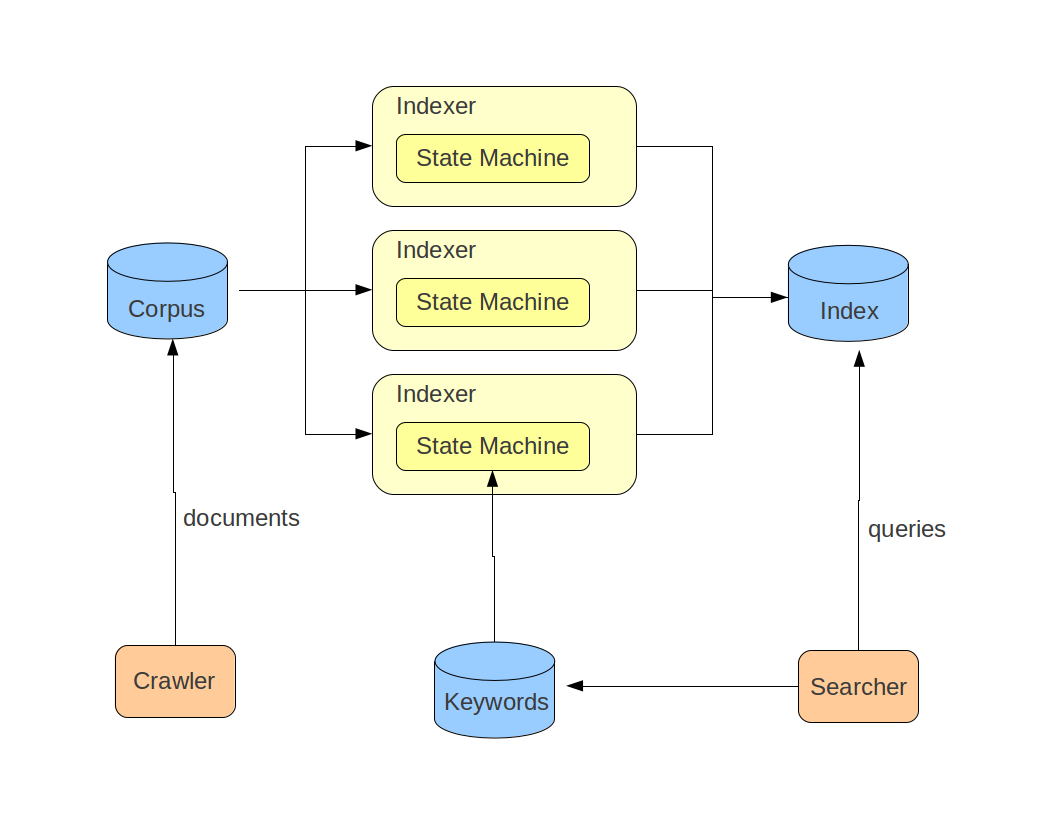
\includegraphics[width=0.70\textwidth,height=!]{deploymentmodel}
  \end{center}
  \caption{Indexer deployment model}
  \label{fig:deploymentmodel}
\end{wrapfigure} 


%----------------------------------------
% Experiment Results
%----------------------------------------
\section{Experiment Results}
\label{sec:experimentresults}
The primary goal of this project is to be able to reduce the time
to build a document index. As our system is building the inverted index by
parsing all documents of the collection, we can expect the
time complexity of the task to be proportional to the sum total of
characters in the collection. As a result, changing the  
number of documents or the average size of each document should
have a big impact in our time complexity. In addition, our
implementation will incur the cost of building the Aho-Corasick state
machines used to scan the documents. We can expect the time to build a
state machine to be proportional to the sum of the size of the
keywords. 

Finally we will do a time comparison between our indexer
implementation and a na\"{i}ve implementation. All the time
complexities tests are done on a single computer and it is important
to understand that all these processes can be parallelized. In section
\ref{parallelization} we install our indexer on multiple computers and
explore the performance gain of running parallel instances
simultaneously.

All tests were run on a single Intel Core 2 Duo 2GHz processor, 1GB
RAM, running a 64-bit Linux 2.6.35 SMP kernel. The Java Virtual
Machine used was version 1.6.0-24. The database used was MySQL,
running on the same node as the indexer.


%----------------------------------------
% Number of Keywords
%----------------------------------------
\subsection{Number of Keywords}
To be able to study the impact of different number of keywords, we
built a keywords database with 10,000 most popular English
words \cite{wordlist}. All the experiments in this
part are done with 50,000 posts randomly downloaded from the Internet. The
idea is to get a good distribution of documents with respect to length
and content. The experiment shown here consist of building the index
for different numbers of keywords from the 10,000 keyword database and
explore the time and space complexity for the building of the state
machine and the building of the index using the state machine.

The time taken to construct the Aho-Corasick state machine was
measured for different numbers of keywords. The results of this test
is shown in figure \ref{fig:numkeywordstimecomplexbuildsm} and
construction time can easily be considered linear with respect to the
number of keywords. This is consistent with \cite{RefWorks:103} which
proves that the state machine construction algorithm is linearly
proportional to the sum of the lengths of the keywords used to
construct the state machine.

The time taken for a state machines to build an inverted index of our
corpus was measured. The test was repeated using state machines
constructed with a varying number of keywords and the results plotted
in figure \ref{fig:numkeywordstimecomplexbuildindex}. According to
\cite{RefWorks:103} which proves that the number of state transitions
involved in processing an input string is independent of the number of
keywords used to construct the state machine, we would not expect the
time complexity to increase with the size of the keyword set. However,
as can be seen in \ref{fig:numkeywordstimecomplexbuildindex}, the time
to build the index increases logarithmically with the number of
keywords. This is likely due to the fact that as the number of
keywords increases, so does the size of the index and the number of
database interacts required to store and update the index.


\begin{figure}[ht]
  \begin{minipage}[b]{0.5\linewidth}
    \centering
    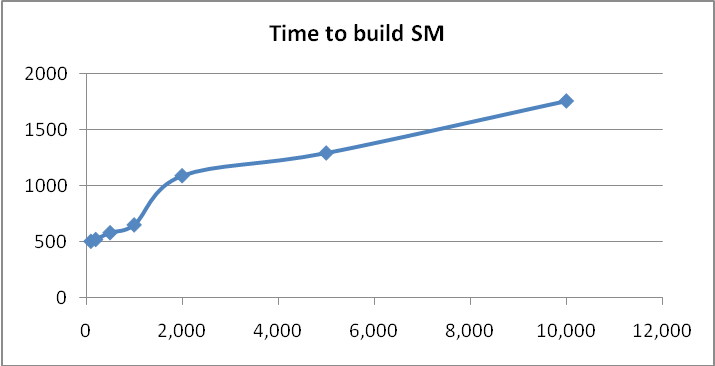
\includegraphics[width=\textwidth]{numkeywordstimecomplexbuildsm}
    \caption{Time to build Aho-Corasick state machine as a function of
      the number of keywords. Time taken is shown in milliseconds on the
      y-axis and the number of keywords on the x-axis}
    \label{fig:numkeywordstimecomplexbuildsm}
  \end{minipage}
  \hspace{0.5cm}
  \begin{minipage}[b]{0.5\linewidth}
    \centering
    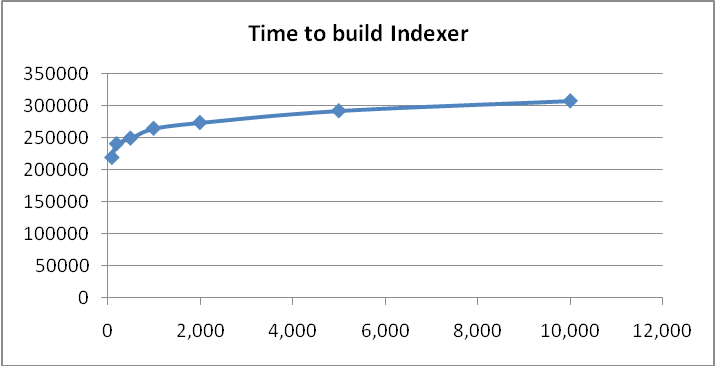
\includegraphics[width=\textwidth]{numkeywordstimecomplexbuildindex}
    \caption{Time to build the inverted index as a function of the
      number of keywords. Time taken is shown in milliseconds on the
      y-axis and the number of keywords on the x-axis}
    \label{fig:numkeywordstimecomplexbuildindex}
  \end{minipage}
\end{figure}

The space used by the index in the database is proportional to the
number of words we are using. It also means that our words have the
same probability at the beginning or at the end of our 12,000 word
dictionary.


%----------------------------------------
% Size of Corpus
%----------------------------------------
\subsection{Size of Corpus}
To be able to study the impact of different number of Posts, we built
a posts database with 400,000 posts randomly downloaded from
the Internet. Then the keywords used to build the index are simply the
first 5,000 from the previous keywords database. 

The experiment shown here consist on building the index for different
number of Posts and explore the time and space complexity for the
building of the state machine and the building of the index once the
state machine is built. We can expect that the time to build the State
machine won’t change with the number of posts and the time to build
the index will increase almost linearly with the number of posts.  

As we were expecting, the time to build the index with the state
machine strategy is linear with respect to the number of post, as
depicted in figure \ref{fig:corpsizetimecomplexbuildindex}. However, to be able
to perform this experiment we had to run the indexer program with
batches of 10,000 posts due to Java heap space problems. As a result, the state
machine is rebuilt every 10,000 posts.  

The space used to store the index in the database is
proportional to the size of the corpus as shown in figure
\ref{fig:corpsizespacecomplexbuildindex}.


\begin{figure}[ht]
  \begin{minipage}[b]{0.5\linewidth}
    \centering
    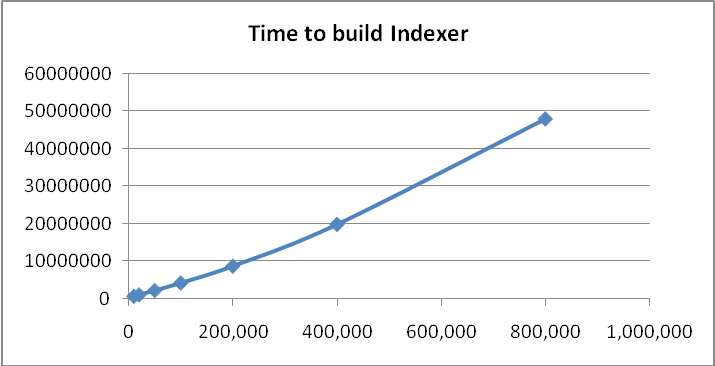
\includegraphics[width=\textwidth]{corpsizetimecomplexbuildindex}
    \caption{Time to build the inverted index as a function of the
      size of the corpus. Time taken is shown in milliseconds on the
      y-axis and the number of documents in the collection on the
      x-axis} 
    \label{fig:corpsizetimecomplexbuildindex}
  \end{minipage}
  \hspace{0.5cm}
  \begin{minipage}[b]{0.5\linewidth}
    \centering
    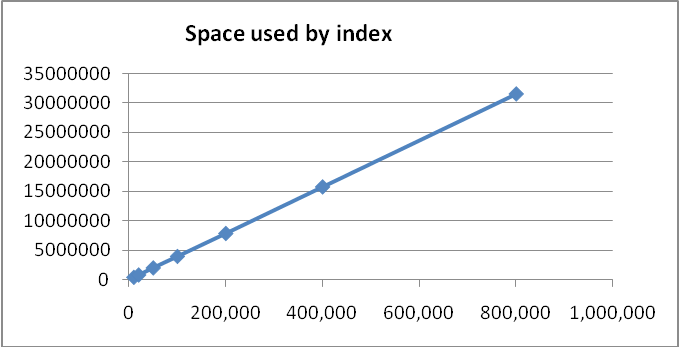
\includegraphics[width=\textwidth]{corpsizespacecomplexbuildindex}
    \caption{Size of index as a function of the size of the
      corpus. The number of database rows used to store the index is
      shown on the y-axis and the number of documents in the
      collection on the x-axis} 
    \label{fig:corpsizespacecomplexbuildindex}
  \end{minipage}
\end{figure}


%----------------------------------------
% Document Size
%----------------------------------------
\subsection{Document Size} 
As we have seen before, the time to build the index is almost
proportional with the number of post. Theoretically this time should
be proportional to the total length of all posts. Let’s focus on this
aspect and study the impact of the length of the post on the time to
build the state machine. To do that we built a 5,000 posts database
with posts that are all composed of 20,000 characters. Then, we ran
our system on different length of substring of these posts. 


\begin{figure}[ht]
  \begin{minipage}[b]{0.5\linewidth}
    \centering
    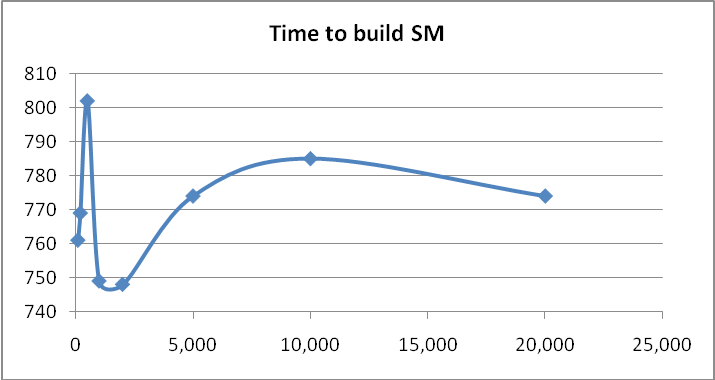
\includegraphics[width=\textwidth]{docsizetimecomplexbuildsm}
    \caption{Time to build Aho-Corasick state machine as a function of
      the average document size. Time taken is shown in milliseconds on the
      y-axis and the average document size in characters on the x-axis}
    \label{fig:docsizetimecomplexbuildsm}
  \end{minipage}
  \hspace{0.5cm}
  \begin{minipage}[b]{0.5\linewidth}
    \centering
    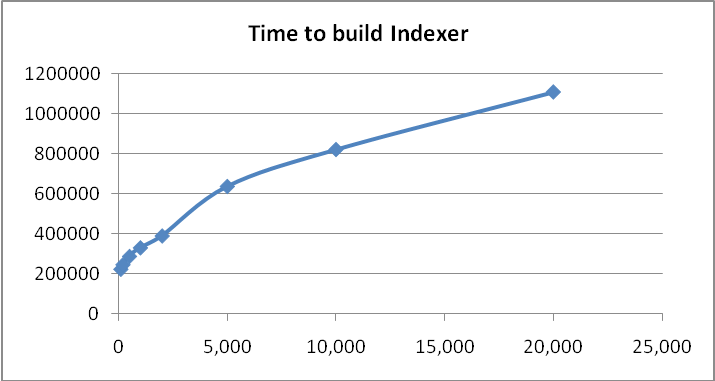
\includegraphics[width=\textwidth]{docsizetimecomplexbuildindex}
    \caption{Time to build an inverted index as a function of the
      average document size. Time taken is shown in milliseconds on the
      y-axis and the average document size in characters on the x-axis} 
    \label{fig:docsizetimecomplexbuildindex}
  \end{minipage}
\end{figure}
 

State machine construction time does not depend on the
length of the documents. Nonetheless it is interesting to compare
figures \ref{fig:docsizetimecomplexbuildsm} and
\ref{fig:docsizetimecomplexbuildindex}, showing the construction times
for the state machine and inverted index relative to the average
document size. The comparison shows that state machine construction
time is several orders of magnitude smaller than index construction
and negligible by comparison. Our state machine is built in 770 ms on
average for 1000 keywords with a standard deviation of 18ms.

As expected the time to build the indexer is almost linear with
respect to the average document size. This relationship is shown in
figure \ref{fig:docsizetimecomplexbuildindex}.

As expected, the larger the documents the more records created to
represent the index. However, the relationship is not linear since if
a word occurs many times in the same post we just save it once in the
database. This relationship is shown in figure
\ref{fig:docsizespacecomplexbuildindex}.


\begin{wrapfigure}{r}{0.70\textwidth}
  \begin{center}
        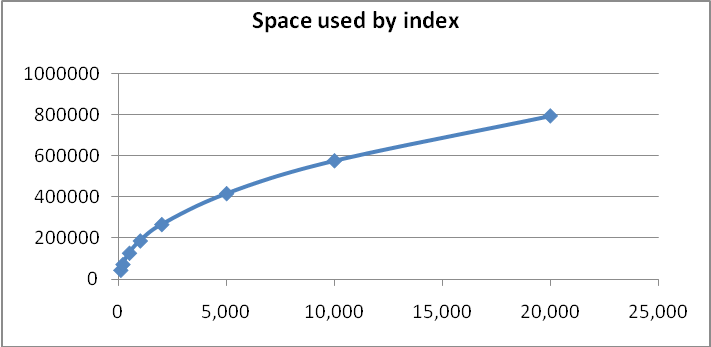
\includegraphics[width=0.70\textwidth,height=!]{docsizespacecomplexbuildindex}
  \end{center}
  \caption{Size of index as a function of the average document
    size. The number of database rows used to store the index is
    shown on the y-axis and the average document size in characters
    on the x-axis}  
  \label{fig:docsizespacecomplexbuildindex}
\end{wrapfigure} 


%----------------------------------------
% Comparison with Naive Index Builder
%----------------------------------------
\subsection{Comparison with Na\"{i}ve Index Builder}
This part focuses on the improvement that our system with respect to
time complexity in comparison with a na\"{i}ve index builder. The na\"{i}ve
indexer builder has the same input as our system i.e. a list of
keywords and a list of documents, and the same output i.e. an inverted
index corresponding to the keywords and documents. Algorithm
\ref{alg:invertedindex} is used in principal for both implementations.


\begin{algorithm}
\caption{Build inverted index}
\label{alg:invertedindex}
\begin{algorithmic}
  \FORALL{$keyword$}
  \STATE Build a vector $v$
  \FORALL {$document$}
  \IF {$keyword$ \epsilon \; $document$}
  \STATE Add the row (keyword.id, document.id) into $v$
  \ENDFOR
  \STATE Save $v$ into the database
  \ENDFOR
\end{algorithmic}
\end{algorithm}

As we can see this algorithm has a complexity that directly depends on
the number of keywords $n$, the number of document $m$, and the length
of document since we have to check in each document for each
keyword. Moreover, we decided to limit, as much as possible, the
accesses to the database since it is really time consuming in
Java. That’s why we do one access to the database for each keywords
and not for each document. In the state machine we do as much accesses
to the database as the number of document (in the worst case meaning
we find at least one keyword per document). In the following
subsections we compare the results for this algorithm with our system
results for different number of keywords and posts.

For the na\"{i}ve algorithm described above, the theoretical worst
case time complexity relationship is shown in equation
\ref{eqn:timecomplexworstcase}.  

\begin{equation}
\label{eqn:timecomplexworstcase}
Time \propto keyNum * ( docNum * maxLength + conn)
\end{equation}

where \(keyNum\) is the number of keywords, \(docNum\) is the number
of documents, \(maxLength\) is the maximum document length, and
\(conn\) is the time taken to create a connection to the database. For
the state machine algorithm the theoretical complexity relationship is
given by equation \ref{eqn:timecomplexsm}.

\begin{equation}
\label{eqn:timecomplexsm}
Time \propto docNum * ( maxLength + conn)
\end{equation}

To exmaine the effect of document size, the number of keywords was
fixed at 1,000 and the number of documents to 5,000 and we ran our
code on a database composed of document of different length. The
experiment results are shown in figure \ref{fig:naivedocumentsize}. As
expected, the curves for both our indexer and the naive indexer are
almost linear since for the naive implementation: 

\[Time \propto (keyNum * docNum) * maxLength + conn * keyNum\]

and for our Aho-Corasick state machine method: 

\[Time \propto docNum * maxLength + conn * docNum\]

We can observe that for a small length of document naive method is
faster since \(keyNum\) is smaller than \(docNum\). For \(docLength = 1300\)
our indexer is far more efficient. To see this effect more clearly,
experiment results are plotted on a logarithmic scale in figure
\ref{fig:naivedocumentsizelog}.As expected, the two implementations
exhibit a linear response to the number of keywords used. In the
na\"{i}ve implemementation:  


\begin{figure}[ht]
  \begin{minipage}[b]{0.5\linewidth}
    \centering
    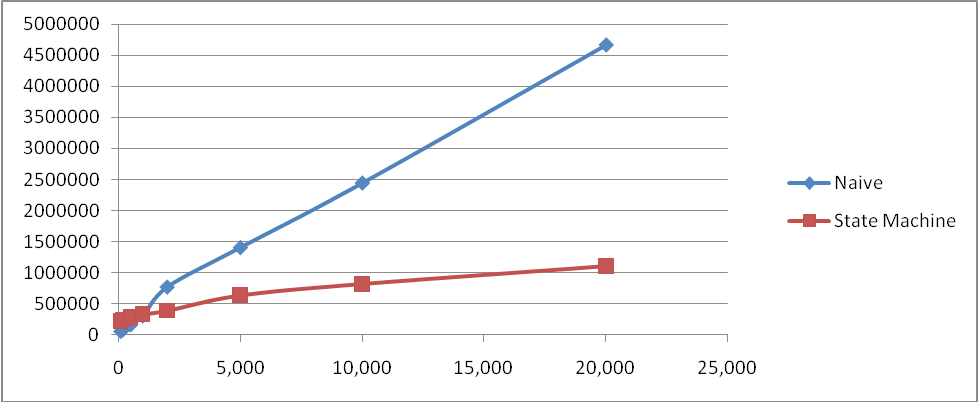
\includegraphics[width=\textwidth]{naivedocumentsize}
    \caption{Time to build an inverted index as a function of the
      average document size. Time taken is shown in miliseconds on the
      y-axis and the average document size in characters on the x-axis}
    \label{fig:naivedocumentsize}
  \end{minipage}
  \hspace{0.5cm}
  \begin{minipage}[b]{0.5\linewidth}
    \centering
    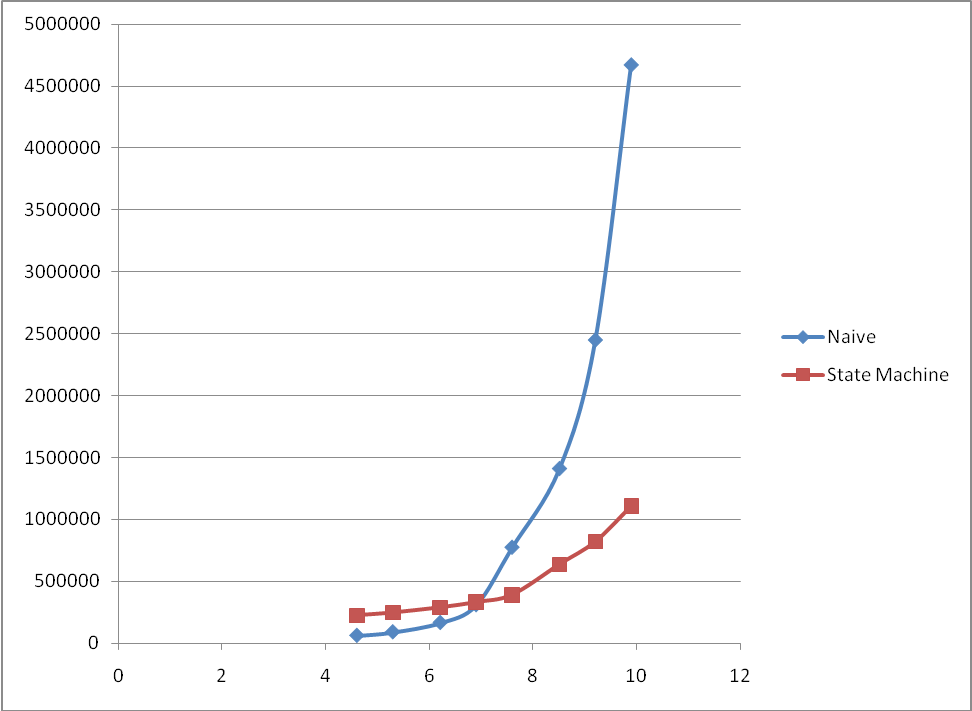
\includegraphics[width=\textwidth]{naivedocumentsizelog}
    \caption{Time to build an inverted index as a function of the
      average document size. Time taken is shown in milliseconds on the
      y-axis and the average document size in characters on the
      logarithmic x-axis}
    \label{fig:naivedocumentsizelog}
  \end{minipage}
\end{figure}


\[Time \propto (keyNum * maxLength) * docNum + conn * keyNum\]

and in our Aho-Corasick state machine method: 

\[Time \propto (maxLength + conn) * docNum \]

However, we would have expected the state machine method not to depend
on the number of keyword. The reason why it’s not the case is because
when we don’t have any keywords in a document, we don’t access the
database. Knowing that the database access is very time consuming,
increasing the number of keyword increases the probability of finding a
keyword into each document and so increase the time complexity.  

The experiment results are shown in figure \ref{fig:naivenumkeywords}
and on a logarithmic scale in figure \ref{fig:naivenumkeywordslog}.


\begin{figure}[ht]
  \begin{minipage}[b]{0.5\linewidth}
    \centering
    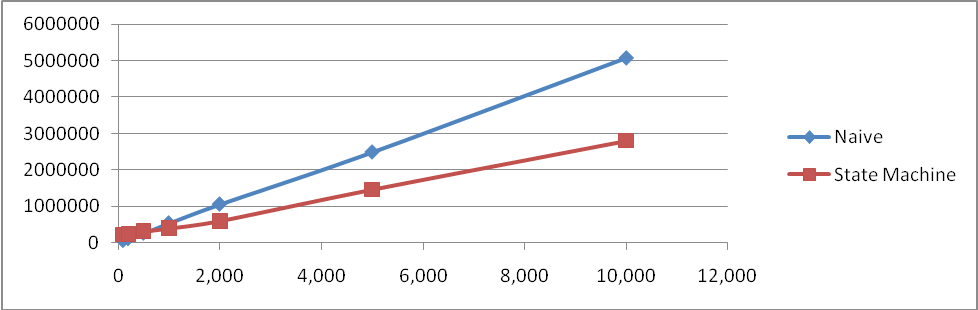
\includegraphics[width=\textwidth]{naivenumkeywords}
    \caption{Time to build an inverted index as a function of the
      number of keywords. Time taken is shown in milliseconds on the
      y-axis and the number of keywords on the x-axis}
    \label{fig:naivenumkeywords}
  \end{minipage}
  \hspace{0.5cm}
  \begin{minipage}[b]{0.5\linewidth}
    \centering
    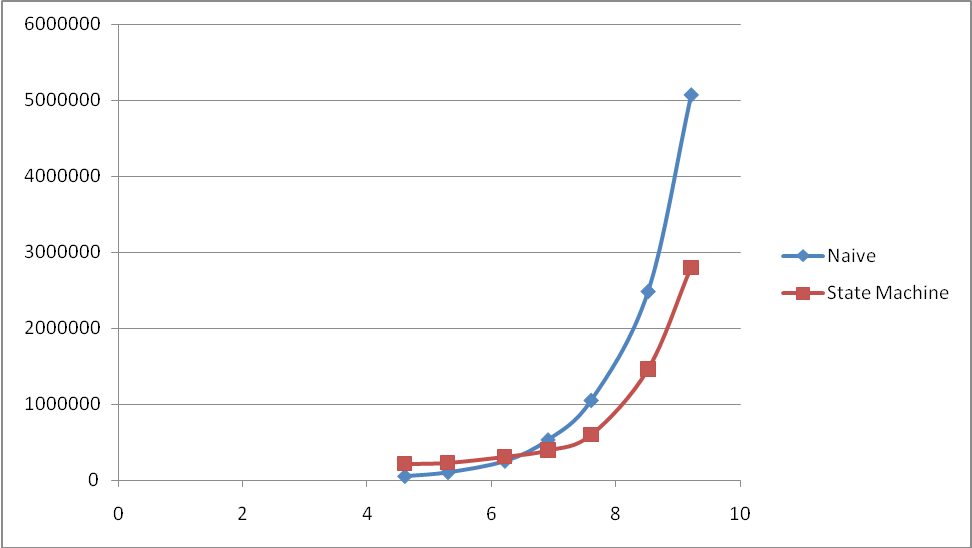
\includegraphics[width=\textwidth]{naivenumkeywordslog}
    \caption{Time to build an inverted index as a function of the
      number of keywords. Time taken is shown in milliseconds on the
      y-axis and the number of keywords on the logarithmic x-axis}
    \label{fig:naivenumkeywordslog}
  \end{minipage}
\end{figure}


As expected, the time complexity is linearly related to the number of
documents being indexed. The experiment results, in this respect, are
shown in figure \ref{fig:naivesizecorpus} and on a logarithmic scale
in figure \ref{fig:naivesizecorpuslog}. For the na\"{i}ve
implementation:

\[Time \propto (docNum * maxLenght + conn) * keyNum\]
 
and in our Aho-Corasick state machine method: 

\[Time \propto docNum * maxLenght + conn * docNum\]


\begin{figure}[ht]
  \begin{minipage}[b]{0.5\linewidth}
    \centering
    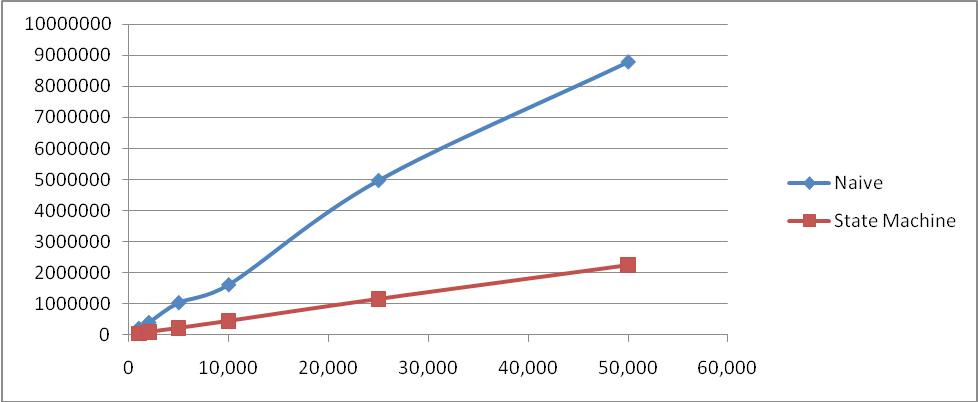
\includegraphics[width=\textwidth]{naivesizecorpus}
    \caption{Time to build an inverted index as a function of the
      number of documents being indexed. Time taken is shown in
      milliseconds on the y-axis and the number of documents on the
      x-axis} 
    \label{fig:naivesizecorpus}
  \end{minipage}
  \hspace{0.5cm}
  \begin{minipage}[b]{0.5\linewidth}
    \centering
    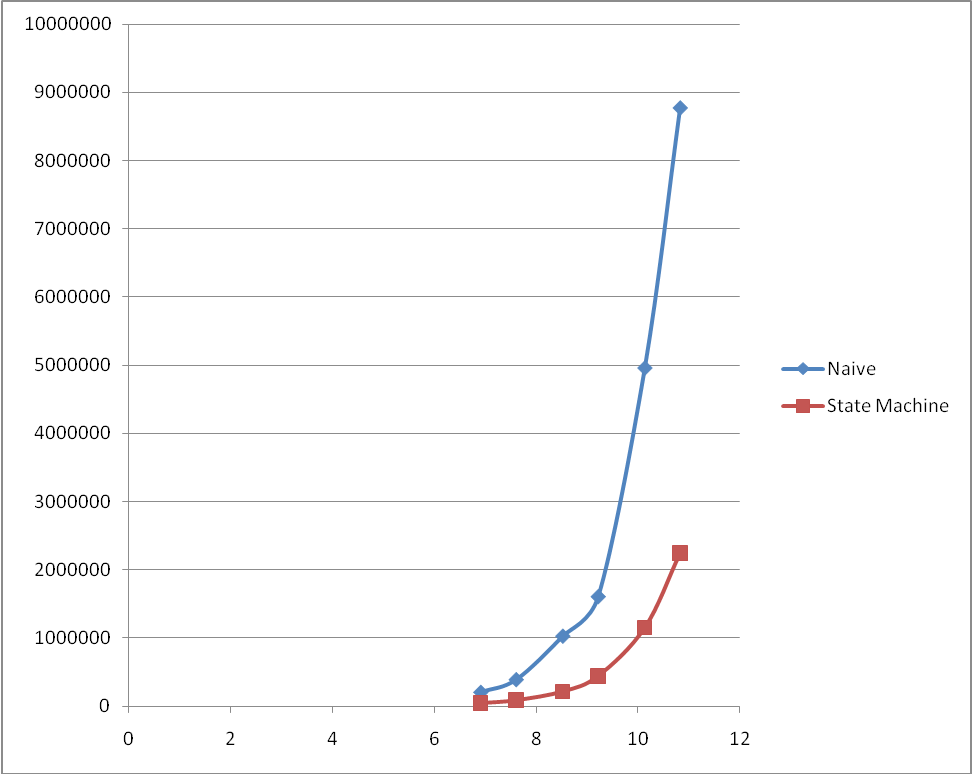
\includegraphics[width=\textwidth]{naivesizecorpuslog}
    \caption{Time to build an inverted index as a function of the
    number of documents being indexed. Time taken is shown in
      milliseconds on the y-axis and the number of documents on the
      logarithmic x-axis} 
  \label{fig:naivesizecorpuslog}
  \end{minipage}
\end{figure}



%----------------------------------------
% Parallelization
%----------------------------------------
\subsection{Parallelization}
\label{parallelization}
Given the modular architecture of our indexer, it is possible to
deploy multiple instances of the program to work concurrently on the same
indexing task. The instances interact via the database which
synchronizes their operations on the corpus and the index itself. To
investigate the effect of parallelization on the indexer operation, the
indexer was deployed using a single database server storing documents,
keywords, and the resulting index; four indexer nodes each running a
single instance of the indexer program. 

In this experiment a corpus of 100,000 documents and 1000 keywords were
used, each document 5000 words in length. Tests were run using various
node combinations and the time taken to index the corpus was measured and
normalized to a throughput metric (documents/second) for convenient
comparison. Test results using the same number of nodes were averaged
to account for differences in the physical capabilities and
configuration of the worker nodes. Next, a series of tests was
performed using a corpus of 800,000 documents to investigate the
effect of corpus size on performance. The results of this experiment
are shown in figure \ref{fig:parallelization}.

For the 100,000 document corpus, increasing the number of nodes
increases throughput but with diminishing returns. As the database
connection pool is saturated, this becomes the limiting factor of the
architecture. If the number of nodes were increased further, one would
expect the curve to plateau at some point. After this point, adding
additional nodes would offer no improvement and may even decrease
performance as the worker processes spend an increasing amount of time
context switching and contending for locks. These factors could be
mitigated up to a point by increasing batch sizes and tuning the
database. However, the characteristics of the curve are ultimately
unavoidable in the current architecture. 

For the 800,000 document corpus, the performance curve shows an even
more severe degradation than the smaller corpus. Since we normalize
the performance metrics for the size of the document collection, one
would expect this curve to be more similar to that of the 100,000
document collection. A possible explanation for the deviation is that
for the larger collection, more documents were present in the
database and the resulting index larger. This results in longer table
scan times to retrieve and update records. This effect could be
alleviated through the use of indices and other database optimization
techniques, however, as for the smaller document
collection, this degradation is ultimately unavoidable.


\begin{wrapfigure}{r}{0.70\textwidth}
  \begin{center}
        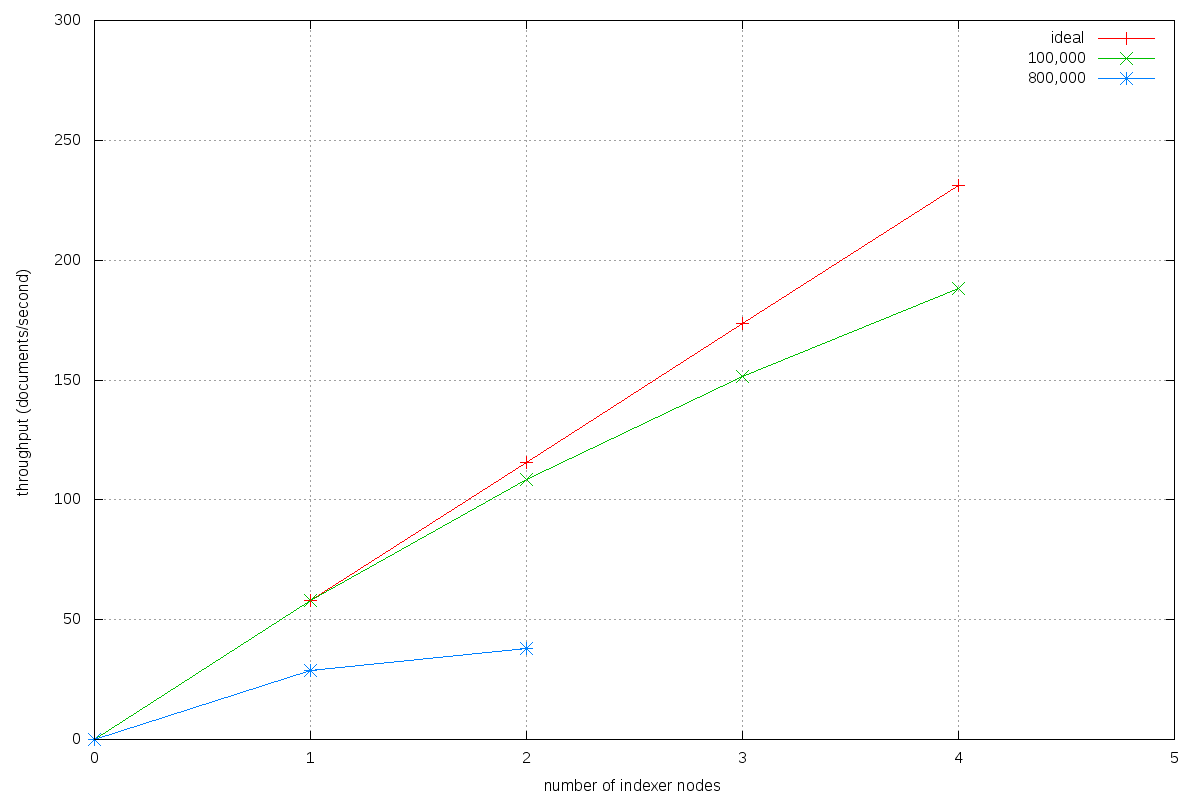
\includegraphics[width=0.60\textwidth,height=!]{parallelization}
  \end{center}
  \caption{Performance characteristics of parallel indexer
    deployment. The \textit{ideal} curve shows the theoretical
    performance curve based on linear combination of average
    individual node performance over the corpus} 
  \label{fig:parallelization}
\end{wrapfigure} 


%----------------------------------------
% Conclusions
%----------------------------------------
\section{Conclusions}
\label{sec:conclusions}
The experimental results tend to prove what we could expect from
theory. Our system is faster than the na\"{i}ve indexer with respect
to the number of keywords being indexed, size of the document
collection, and average document size. In particular, our indexer
implementation performs relatively well with respect to the number of
documents being indexed. Moreover, as soon as we are dealing with a number of
keywords that can be representative of real-world needs, the state
machine implementation proves also to be significantly faster than the
naive indexer. 

One of the primary goals of this research project was to leverage the
effect of parallelization in reducing the time to index a document
collection. We successfully demonstrated that performance gains could
be achieved for the indexing task through parallelization as well as
the fact that our architecture offers diminishing returns as the
number of nodes is increased and as the corpus becomes larger.

 Other avenues of interest include, but are not limited
to:

\begin{itemize}
  \item Compare the Aho-Corasick state machine indexer implementation
    to less na\"{i}ve indexer implementations.
    
    \item Use compression techniques to our algorithm in order to
      reduce the index size in the database.

      \item Conduct further parallelization experiments to determine
        the performance characteristics of our indexer over a wider
        range of operating conditions.

    \item Study the time performance improvements possible deploying
      the Aho-Corasick state machine indexer within a commercial
      \textit{MapReduce} framework such as \textit{Hadoop}.
\end{itemize}



%----------------------------------------
% Bibliography
%----------------------------------------
% changes default name Bibliography to References
\renewcommand\bibname{References}
\bibliography{bibliography}
\bibliographystyle{IEEEannot}

\end{document}
